%--------Visión General de la Solución
%--------Daniel Ochoa John
%--------05/06/2012

\chapter{Visión general de la solución}
\label{cap:vision}
En este capítulo se describe conceptualmente la solución desarrollada en este trabajo de tesis. En primer lugar, se expone el modelamiento que fundamenta el desarrollo de los distintos componentes de \textit{software} que este trabajo presenta. Posteriormente, se describe el mecanismo de \textit{community \textit{cache}} detonado al momento de recomendar. Luego, se explica cómo esos conceptos son transformados en un modelamiento de \textit{software}.  Finalmente, se muestra la integración entre los distintos componentes con apoyo de un diagrama general de la solución.

\section{Modelamiento}
\label{vision:redes}

En esta sección se detalla el modelamiento de los distintos aspectos involucrados en el desarrollo de este trabajo de tesis. El modelamiento sienta las bases sobre las que la solución es construída. En otras palabras, el resultado de este ejercicio conforma los requisitos funcionales que la solución debe contemplar. 

\subsection{Modelamiento de interacciones}

Como ya se ha mencionado anteriormente, en un contexto de social media pueden ocurrir diversas interacciones, como un mensaje, un ‘me gusta’, un follow, entre otras. En una red social hay diversas interacciones y depende del contexto y del dominio la relevancia de cada una de ellas en relación a su consideración en una recomendación hacia un usuario activo.

Son estas interacciones las que denotan a una comunidad. Por ejemplo, si en un contexto de una tienda virtual, un usuario realiza una valoración (\textit{rating}) mediante el método que fuere, como por ejemplo una valoración de un artículo en una escala del uno al cinco, dicha valoración será considerada, de una u otra manera, al momento de recomendar aquel artículo a otro usuario que pertenezca a la misma comunidad.

No obstante, diferentes interacciones pueden denotar muchos segmentos de interés para un usuario. Hipotéticamente hablando, si se considera un contexto de social media en el que sólo existen dos posibles interacciones: amistad y \textit{following}, es posible que un usuario establezca una interacción de amistad con personas que conozca físicamente o virtualmente. No obstante, es posible que genere eventos de \textit{following} con personas relacionadas con temas en boga, como una noticia importante, algún evento deportivo, entre otras. Ante esto pueden ocurrir dos situaciones principales, que los segmentos o comunidades de interés denotadas por ambas interacciones para un usuario sean similares, o que ambas interacciones determinen segmentos de interés divergentes entre sí.

En RBox, las interacciones son modeladas a través de eventos, siguiendo las directrices establecidas por el meta modelo de la 3-Ontology. Pragmáticamente, existe una interfaz llamada Event (ver Figura \ref{fig:vis-im1}), que define este meta modelo. Por lo que todo evento debe tener un valor y contextualmente debe ser realizado por un usuario, enfocado en un objeto en particular (que puede ser otro usuario), situado en una comunidad, realizado en un lugar en particular y debe contar con una marca temporal. 

\begin{figure}
  \centering
  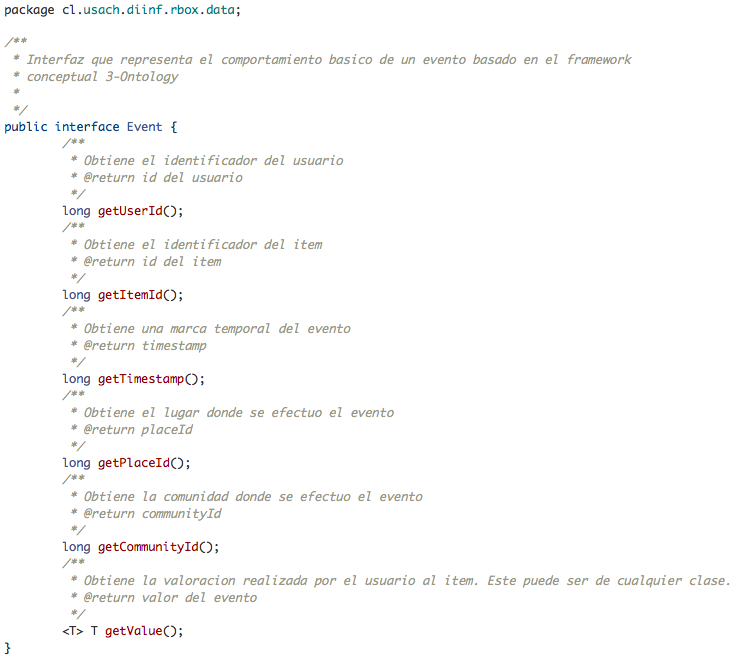
\includegraphics[scale=.5]{images/Figura7-1}
  \caption{\em Interfaz Event del código fuente de RBox.}
  \label{fig:vis-im1}
\end{figure}

Entonces, uno de los problemas que deben ser resueltos en la implementación de la solución es el de realizar una correspondencia entre el modelo de datos del dominio situado en un ambiente de social media y una definición de evento tipada por RBox.

\subsection{Modelamiento de la detección de comunidades}

En ese sentido y considerando lo anterior, es que la detección de comunidades que la solución provea debe considerar a aquellas que están latentes en el dominio de los distintos eventos. Por ende, es necesario abstraer el concepto de evento de manera tal que la solución sea capaz de detectar comunidades en base a todas aquellas interacciones que sean definidas como relevantes para un cierto dominio de análisis. 

En el mundo de la tecnología (y de los repositorios de código) existen distintas librerías que implementan mecanismos y técnicas para detectar comunidades que existen en la literatura:

\begin{itemize}
	\item Gephi (gephi.github.io/)
	\item igraph (igraph.org/)
	\item graph-tool (graph-tool.skewed.de/)
	\item JGraphT (jgrapht.org/)
	\item GraphStream (graphstream-project.org/)
	\item entre otras ... 
\end{itemize}

Su uso, en desmedro de implementar los algoritmos desde su publicación, tiene la tiene la gran ventaja de contar con una comunidad que respalda su uso, funcionamiento, resultados y que además hace el código mantenible.

No obstante, es claro notar que estas librerías, o APIs, están enfocadas en un modelamiento en base a grafos, en donde los nodos representan a los usuarios de una red social y las aristas representan una conexión (a partir de interacciones, según la red social) entre dos usuarios. Por ende, otro de los problemas que deben ser resueltos por la solución presentada por este trabajo, es el de encapsular la información contenida por las distintas instancias de los objetos que pertenezcan una clase que implemente la interfaz Event, con el objetivo de generar un grafo de interacciones.

Al contar con un grafo de interacciones, es posible utilizar las APIs disponibles para análisis de grafos (la detección de comunidades incluida) con el objetivo de detectar las comunidades latentes, que existen en aquel grafo.

\subsection{La 3-Ontology y las comunidades}

Las comunidades son una dimensión considerada en el meta modelo de la 3-Ontology y está definida en el \textit{framework} de RBox como muestra el código de la Figura \ref{fig:vis-im2}. Una comunidad, entonces, está formada principalmente por un conjunto de usuarios. Cuando se hace uso de la detección de comunidades, se debe contar con un mecanismo o componente que sea capaz de integrar los dos mundos: el de la teoría de grafos con el correspondiente a la 3-Ontology.

\begin{figure}
  \centering
  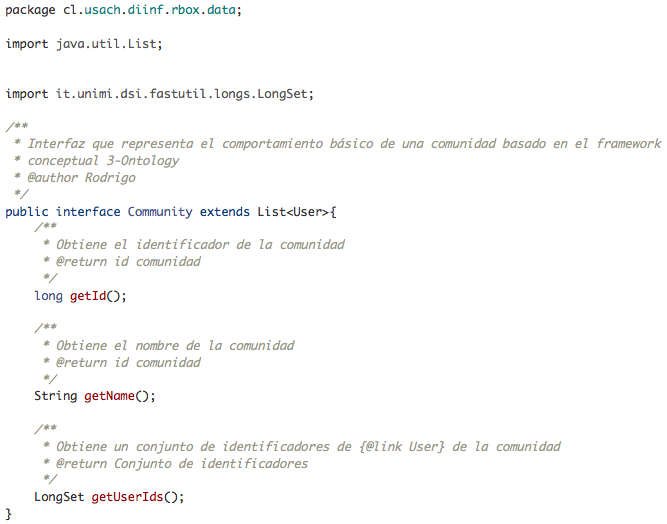
\includegraphics[scale=.5]{images/Figura7-2}
  \caption{\em Interfaz Community del código fuente de RBox.}
  \label{fig:vis-im2}
\end{figure}

Como se ha mencionado en la sección anterior, el componente que sea responsable de manejar la detección de comunidades, estará trabajando bajo un dominio de la teoría de grafos y no necesariamente debe inmiscuirse con el meta modelo planteado por la 3-Ontology. Esto fundamentado en el principio de única responsabilidad (single responsibility principle, en inglés) en la ingeniería de \textit{software} (Martin, 2003), el cual plantea que cada componente de una aplicación debe responder a un propósito atómico e independiente. En ese sentido, la detección de comunidades puede ser considerado un propósito independiente del proceso o \textit{framework} que haga uso de sus beneficios. 
    
Lo anterior genera una arista adicional a considerar en el diseño de la solución que es, precisamente, la integración entre los dos mundos. Debe existir un componente, herramienta o librería que sea capaz de realizar una transformación desde la meta información que contiene un grafo con comunidades detectadas, hasta un esquema definido en base a las directrices que plantea la 3-Ontology, es decir, pasar de un conjunto de nodos y aristas pertenecientes a un \textit{‘cluster’}, hacia una comunidad, que contiene un conjunto de usuarios.

\section{Community Cache}

El objetivo principal de este trabajo es verificar si contar con un mecanismo de \textit{‘\textit{cache}’} para manejar las comunidades en ejecuciones previas de un sistema de recomendación, permite mejorar el tiempo de respuesta que es requerido para otorgar una recomendación a un usuario activo. En ese contexto, es necesario definir el mecanismo de \textit{cache} que será construído y como actúa en el flujo actual de la recomendación, planteado por el \textit{framework} RBox.

Este flujo considera (de izquierda a derecha en la Figura \ref{fig:vis-im3}) , precisamente, un \textit{mapping} desde una red social hacia la lógica de la 3-Ontology. Posteriormente, para un usuario activo se tiene definición de los contenedores de sentido: comunidades, eventos y lugares. Luego, y al momento de realizar una recomendación, se toma en cuenta aquellos contenedores de sentido tipificados por distintos factores, como el contexto temporal en el que fueron realizados, como por ejemplo, lugares visitados entre una fecha y otra.

\begin{figure}
  \centering
  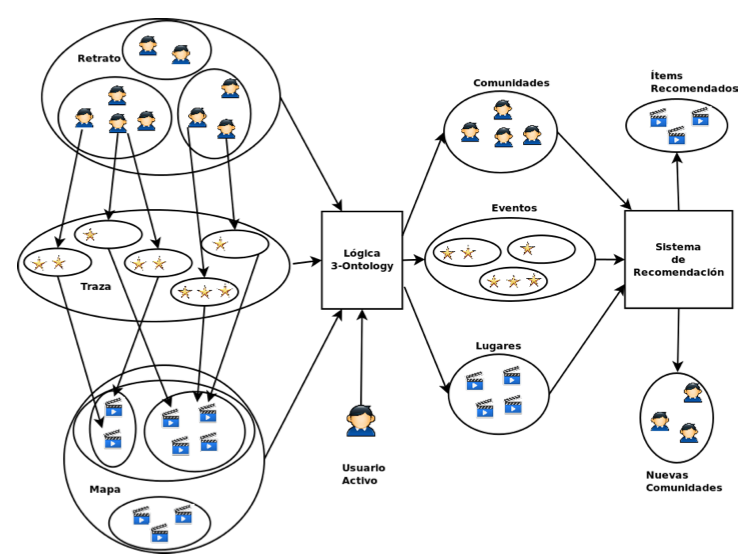
\includegraphics[scale=.5]{images/Figura7-3}
  \caption{\em Flujo propuesto por RBox para llevar a cabo una recomendación.}
  \label{fig:vis-im3}
\end{figure}

Lo anterior da como resultado un conjunto de ítems recomendados, así como también nuevas comunidades. Son estas comunidades las que deben ser persistidas y, de esta manera, estar disponibles para su uso como retroalimentación hacia recomendaciones posteriores. Una \textit{cache} es necesaria debido a que cabe la posibilidad de que las comunidades detectadas en distintas iteraciones del algoritmo de recomendación ya hayan sido detectadas en iteraciones precedentes, por lo que su manejo debe ser tratado con mayor ligereza que aquellas que son detectadas por primera vez. El concepto de ligereza en el manejo de las comunidades pasa por incorporar al mecanismo de \textit{cache} dos niveles de manejo: uno que faculte la activación o no de la detección de comunidades en una recomendación y otro que maneje, de cierta forma, las distintas apariciones de las comunidades detectadas.

\subsection{Primer nivel de \textit{cache}}

El primer nivel de \textit{cache} considera un mecanismo para enfrentar el escenario en el cual no existen comunidades detectadas para un usuario. Si el contexto de social media en el que un recomendador esté funcionando no considera de manera explícita el concepto de comunidad (por ejemplo, Google+ si lo hace), entonces en el esquema de la 3-Ontology, los usuarios no tendrían comunidades asociadas en primera instancia.

No obstante, lo anterior no quiere decir que estas no existan, por lo que se define un mecanismo que active la detección de comunidades si un usuario activo no pertenece a ninguna comunidad. En el caso de redes sociales de \textit{microblogging}, como Twitter, las comunidades no son explícitas y la gran cantidad de tópicos que son tratados (y a la velocidad que son tratados), implica que un usuario puede estar inmerso en distintas comunidades, de manera implícita.

Esto puede tener un impacto en el tiempo requerido para realizar una recomendación. Ciertamente, el proceso de detección de comunidades durante la generación de una recomendación, representa un costo de tiempo adicional. A esto hay que agregar el tiempo requerido para operaciones de persistencia, como lectura y escritura de una base de datos, por ejemplo.

Luego, el primer nivel de \textit{cache} permite establecer una estrategia de detección de comunidades, en la que, por ejemplo, se puede utilizar un proceso que, luego de cierto tiempo planificado, desactive el primer nivel de \textit{cache}, con la finalidad de actualizar las comunidades a las que pertenece un usuario. Esto en desmedro de realizar la detección de comunidades de manera recurrente y cada vez que una aplicación lo requiera.

\subsection{Segundo nivel de \textit{cache}}

El segundo nivel de \textit{cache} es un mecanismo de manejo de las comunidades ya detectadas. Lo que se busca es mitigar, de cierta forma, el aumento en el tiempo necesario para realizar una recomendación considerando detección de comunidades. Si se asume que una comunidad puede ser detectada más de una vez, en más de una iteración del algoritmo de recomendación, entonces lo que se debe hacer es identificar que esa comunidad ya existe.

Cuando una comunidad ya ha sido detectada en iteraciones anteriores del algoritmo, no deben ocurrir las operaciones de persistencia. Se debe evaluar si una comunidad detectada (C’) existe en el medio persistente (C) comparando al conjunto de usuarios (u) que éstas contienen.  Si ambos conjuntos, digamos Cu y C’u son iguales, entonces las comunidades son iguales (\textit{hit}) y la persistencia de la comunidad detectada debe omitirse. En caso contrario (\textit{miss}), las operaciones de persistencia para la comunidad detectada deben ejecutarse.

Lo que se pretende es provocar un efecto de reducción de tiempo al mediano plazo. Lógicamente, en las primeras iteraciones del algoritmo, la cantidad de \textit{hits} será menor a la cantidad de \textit{miss} al momento de evaluar la persistencia de una comunidad detectada. No obstante, a medida que las recomendaciones ocurran, es posible que el proceso de detección de comunidades arroje resultados que ya han ocurrido en iteraciones anteriores, por lo que el mecanismo de persistencia para esa comunidad no será efectuado. Luego, se ahorra el tiempo requerido para ello y la recomendación ocurrirá más rápido.

\section{Componentes de \textit{software}}

En las secciones anteriores se realizó un análisis de aquellas dificultades y consideraciones que debe tener la solución. En esta sección se analizarán las características y responsabilidades que deben tener los componentes de \textit{software}, que serán desarrollados con la finalidad de superar aquellas dificultades y manejar aquellas consideraciones.

\subsection{Manejo de las interacciones}

En primer lugar, deben manejarse adecuadamente las interacciones que existen en un ambiente de social media, con el fin de abordar el problema de correspondencia entre el modelo de datos del dominio y la definición de evento tipada por RBox. En ese sentido, debe existir un componente de \textit{software} que permite realizar un mapeo entre estos dos dominios y exportar hacia un medio persistente la información de las interacciones realizadas por los usuarios.

Este componente debe conectarse al ambiente de social media a través del método más “limpio” posible. Es decir, si el ambiente cuenta con una API disponible para acceder a su información, este método debe ser preferido por sobre otros, como por ejemplo adoptar una estrategia de scrapping.

La estrategia de extracción debe considerar la mayor cantidad de información que las políticas de privacidad de los ambientes permitan y debe tender a completar lo más posible el modelamiento de datos utilizado por RBox, y que está basado en el marco otorgado por la 3-Ontology.

Por otro lado, se deben definir las interacciones del dominio de extracción en RBox. Esto pasa por identificar, tipificar y crear una jerarquía de clases de manera tal que cada una de las interacciones que ocurren en un dominio determinado, deben corresponder, en RBox, a una clase que herede de Evento.

\subsection{Detección de comunidades}

En segundo lugar, debe existir un componente de \textit{software} que otorgue funcionalidad de detección de comunidades. Este componente debe ser construído de manera tal que su integración con RBox no sea invasiva, permitiendo su reemplazo por otros componentes similares, según se requiera.

Como parte de la integración, debe ser abordado el problema de encapsulación de los distintos eventos definidos en RBox, con el objetivo de generar un grafo de interacciones. Este grafo de interacciones debe ser genérico y no debe importar el evento que propicie su construcción. Luego, el componente de \textit{software} debe ser capaz de interpretar este grafo de interacciones y debe proveer diversos mecanismos para realizar detección de comunidades. La respuesta de este componente debe ser un grafo con sus comunidades explicitadas.

\subsection{Persistencia de comunidades}

En tercer lugar, debe existir un componente de \textit{software} que maneje la persistencia de las comunidades detectadas. Entre las responsabilidades de este componente está la de conectarse con el componente de detección de comunidades, incorporando a RBox un servicio que faculte a todo sistema de recomendación desarrollado con el \textit{framework}, el uso de la detección de comunidades.

Uno de los principales desafíos que aborda este componente es el de implementar el mecanismo de \textit{community \textit{cache}} descrito en la sección anterior. Este mecanismo se debe detonar cuando comiencen las operaciones que tengan relación con la persistencia de las comunidades.

La persistencia ocurre al momento de interpretar y transformar desde el grafo con comunidades explicitadas, que es salida del componente de detección de comunidades, hacia el modelo de comunidades que maneja RBox. Es en este momento cuando deben añadirse operaciones al DAO de RBox para que sea capaz de detectar comunidades con un conjunto de usuarios idénticos.

Además, este componente debe integrarse a RBox implementando todos aquellos servicios de DAO que tengan relación con el manejo de las comunidades y que en su primera versión se han dejado sin implementar. Esto con el objetivo de completar el conjunto de herramientas que el API de RBox provee a los desarrolladores de sistemas de recomendación.

\section{Integración de componentes}

Los componentes descritos anteriormente deben integrarse de diversas maneras. La Figura \ref{fig:vis-im4} muestra un diagrama que representa conceptualmente esta integración, entre paréntesis están descritos los nombres de referencia que aparecen en la Figura. En primer lugar está el componente (\textit{\textit{mapping} component}), que resuelve la extracción de interacciones y sus transformaciones a eventos.

\begin{figure}
  \centering
  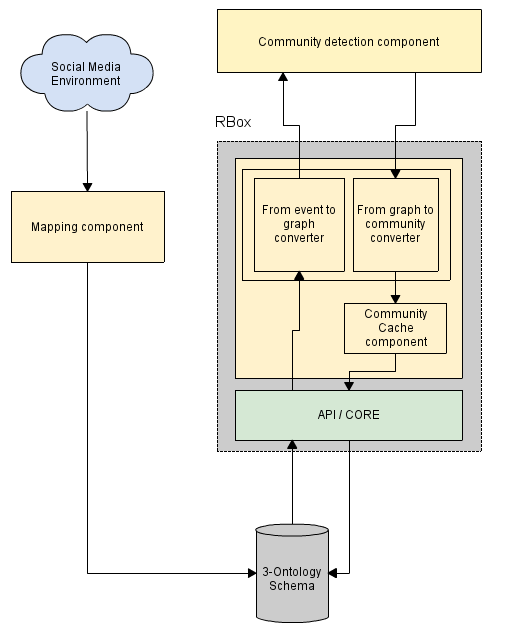
\includegraphics[scale=.5]{images/Figura7-4}
  \caption{\em Diagrama conceptual de integración de los componentes de \textit{software}.}
  \label{fig:vis-im4}
\end{figure}

Este componente extrae información desde el ambiente de social media (\textit{social media environment}) a través del mecanismo más limpio como ya se mencionó anteriormente y persiste estas interacciones en un medio persistente, cuyo esquema está en regla con el definido por la 3-Ontology (3-Ontology \textit{Schema}).

Con el medio persistente ya con eventos, y suponiendo que se está en proceso de recomendación, el componente que convierte los eventos a grafos (\textit{From event to graph converter}), a través de las operaciones de DAO definidas en el API y el CORE de RBox, extrae aquellos eventos que sean de interés y construye un grafo de interacciones.

Posteriormente, este grafo de interacciones es enviado al componente de detección de comunidades (\textit{Community detection component}), que interpreta el grafo, lo procesa y detecta las comunidades mediante un método que le es definido.

Este último componente retorna la información del grafo con comunidades hacia un componente de transformación de grafos a comunidades (\textit{From graph to community converter}) que interpreta este grafo en el esquema definido por la 3-Ontology para las comunidades.

Luego, se procede a las operaciones de persistencia de las comunidades detectadas, por lo que se da inicio a la intervención del componente que maneja la \textit{community \textit{cache}}, quién filtra las comunidades ya persistidas. Esto permite que, luego y nuevamente por operaciones del DAO, se persistan aquellas comunidades detectadas en la ejecución actual del algoritmo de recomendación. Finalmente, se prosigue con la ejecución del algoritmo con normalidad.

\section{Resumen}

En este capítulo se han abordado los desafíos y problemáticas derivadas del cumplimiento del objetivo general de este trabajo de tesis. Se  han descrito aquellos componentes que deben ser incorporados a RBox con la finalidad de proveer una plataforma tecnológica que permite probar la hipótesis propuesta. En los capítulos siguientes se describe con mayor detalle a los componentes de \textit{software} diseñados en este capítulo, con sus implementaciones concretas, arquitecturas y paradigmas utilizados.























